\documentclass[final,nocolorBG,a4,marieke,nototal,pdf, accumulate,slideColor]{prosper}

\addtolength{\textheight}{-1cm}

\usepackage{pstricks,pst-node,pst-text,pst-3d}
\usepackage{amsmath}
\usepackage{alltt}
\usepackage{epsfig}

\usepackage{colordvi}
\usepackage{proof}
\usepackage{epsf}
\usepackage{amssymb}

\message{<Paul Taylor's Proof Trees, 2 August 1996>}
%% Build proof tree for Natural Deduction, Sequent Calculus, etc.
%% WITH SHORTENING OF PROOF RULES!
%% Paul Taylor, begun 10 Oct 1989
%% *** THIS IS ONLY A PRELIMINARY VERSION AND THINGS MAY CHANGE! ***
%%
%% 2 Aug 1996: fixed \mscount and \proofdotnumber
%%
%%      \prooftree
%%              hyp1            produces:
%%              hyp2
%%              hyp3            hyp1    hyp2    hyp3
%%      \justifies              -------------------- rulename
%%              concl                   concl
%%      \thickness=0.08em
%%      \shiftright 2em
%%      \using
%%              rulename
%%      \endprooftree
%%
%% where the hypotheses may be similar structures or just formulae.
%%
%% To get a vertical string of dots instead of the proof rule, do
%%
%%      \prooftree                      which produces:
%%              [hyp]
%%      \using                                  [hyp]
%%              name                              .
%%      \proofdotseparation=1.2ex                 .name
%%      \proofdotnumber=4                         .
%%      \leadsto                                  .
%%              concl                           concl
%%      \endprooftree
%%
%% Within a prooftree, \[ and \] may be used instead of \prooftree and
%% \endprooftree; this is not permitted at the outer level because it
%% conflicts with LaTeX. Also,
%%      \Justifies
%% produces a double line. In LaTeX you can use \begin{prooftree} and
%% \end{prootree} at the outer level (however this will not work for the inner
%% levels, but in any case why would you want to be so verbose?).
%%
%% All of of the keywords except \prooftree and \endprooftree are optional
%% and may appear in any order. They may also be combined in \newcommand's
%% eg "\def\Cut{\using\sf cut\thickness.08em\justifies}" with the abbreviation
%% "\prooftree hyp1 hyp2 \Cut \concl \endprooftree". This is recommended and
%% some standard abbreviations will be found at the end of this file.
%%
%% \thickness specifies the breadth of the rule in any units, although
%% font-relative units such as "ex" or "em" are preferable.
%% It may optionally be followed by "=".
%% \proofrulebreadth=.08em or \setlength\proofrulebreadth{.08em} may also be
%% used either in place of \thickness or globally; the default is 0.04em.
%% \proofdotseparation and \proofdotnumber control the size of the
%% string of dots
%%
%% If proof trees and formulae are mixed, some explicit spacing is needed,
%% but don't put anything to the left of the left-most (or the right of
%% the right-most) hypothesis, or put it in braces, because this will cause
%% the indentation to be lost.
%%
%% By default the conclusion is centered wrt the left-most and right-most
%% immediate hypotheses (not their proofs); \shiftright or \shiftleft moves
%% it relative to this position. (Not sure about this specification or how
%% it should affect spreading of proof tree.)
%
% global assignments to dimensions seem to have the effect of stretching
% diagrams horizontally.
%
%%==========================================================================

\def\introrule{{\cal I}}\def\elimrule{{\cal E}}%%
\def\andintro{\using{\land}\introrule\justifies}%%
\def\impelim{\using{\Rightarrow}\elimrule\justifies}%%
\def\allintro{\using{\forall}\introrule\justifies}%%
\def\allelim{\using{\forall}\elimrule\justifies}%%
\def\falseelim{\using{\bot}\elimrule\justifies}%%
\def\existsintro{\using{\exists}\introrule\justifies}%%

%% #1 is meant to be 1 or 2 for the first or second formula
\def\andelim#1{\using{\land}#1\elimrule\justifies}%%
\def\orintro#1{\using{\lor}#1\introrule\justifies}%%

%% #1 is meant to be a label corresponding to the discharged hypothesis/es
\def\impintro#1{\using{\Rightarrow}\introrule_{#1}\justifies}%%
\def\orelim#1{\using{\lor}\elimrule_{#1}\justifies}%%
\def\existselim#1{\using{\exists}\elimrule_{#1}\justifies}

%%==========================================================================

\newdimen\proofrulebreadth \proofrulebreadth=.05em
\newdimen\proofdotseparation \proofdotseparation=1.25ex
\newdimen\proofrulebaseline \proofrulebaseline=2ex
\newcount\proofdotnumber \proofdotnumber=3
\let\then\relax
\def\hfi{\hskip0pt plus.0001fil}
\mathchardef\squigto="3A3B
%
% flag where we are
\newif\ifinsideprooftree\insideprooftreefalse
\newif\ifonleftofproofrule\onleftofproofrulefalse
\newif\ifproofdots\proofdotsfalse
\newif\ifdoubleproof\doubleprooffalse
\let\wereinproofbit\relax
%
% dimensions and boxes of bits
\newdimen\shortenproofleft
\newdimen\shortenproofright
\newdimen\proofbelowshift
\newbox\proofabove
\newbox\proofbelow
\newbox\proofrulename
%
% miscellaneous commands for setting values
\def\shiftproofbelow{\let\next\relax\afterassignment\setshiftproofbelow\dimen0 }
\def\shiftproofbelowneg{\def\next{\multiply\dimen0 by-1 }%
\afterassignment\setshiftproofbelow\dimen0 }
\def\setshiftproofbelow{\next\proofbelowshift=\dimen0 }
\def\setproofrulebreadth{\proofrulebreadth}

%=============================================================================
\def\prooftree{% NESTED ZERO (\ifonleftofproofrule)
%
% first find out whether we're at the left-hand end of a proof rule
\ifnum  \lastpenalty=1
\then   \unpenalty
\else   \onleftofproofrulefalse
\fi
%
% some space on left (except if we're on left, and no infinity for outermost)
\ifonleftofproofrule
\else   \ifinsideprooftree
        \then   \hskip.5em plus1fil
        \fi
\fi
%
% begin our proof tree environment
\bgroup% NESTED ONE (\proofbelow, \proofrulename, \proofabove,
%               \shortenproofleft, \shortenproofright, \proofrulebreadth)
\setbox\proofbelow=\hbox{}\setbox\proofrulename=\hbox{}%
\let\justifies\proofover\let\leadsto\proofoverdots\let\Justifies\proofoverdbl
\let\using\proofusing\let\[\prooftree
\ifinsideprooftree\let\]\endprooftree\fi
\proofdotsfalse\doubleprooffalse
\let\thickness\setproofrulebreadth
\let\shiftright\shiftproofbelow \let\shift\shiftproofbelow
\let\shiftleft\shiftproofbelowneg
\let\ifwasinsideprooftree\ifinsideprooftree
\insideprooftreetrue
%
% now begin to set the top of the rule (definitions local to it)
\setbox\proofabove=\hbox\bgroup$\displaystyle % NESTED TWO
\let\wereinproofbit\prooftree
%
% these local variables will be copied out:
\shortenproofleft=0pt \shortenproofright=0pt \proofbelowshift=0pt
%
% flags to enable inner proof tree to detect if on left:
\onleftofproofruletrue\penalty1
}

%=============================================================================
% end whatever box and copy crucial values out of it
\def\eproofbit{% NESTED TWO
%
% various hacks applicable to hypothesis list 
\ifx    \wereinproofbit\prooftree
\then   \ifcase \lastpenalty
        \then   \shortenproofright=0pt  % 0: some other object, no indentation
        \or     \unpenalty\hfil         % 1: empty hypotheses, just glue
        \or     \unpenalty\unskip       % 2: just had a tree, remove glue
        \else   \shortenproofright=0pt  % eh?
        \fi
\fi
%
% pass out crucial values from scope
\global\dimen0=\shortenproofleft
\global\dimen1=\shortenproofright
\global\dimen2=\proofrulebreadth
\global\dimen3=\proofbelowshift
\global\dimen4=\proofdotseparation
\global\count255=\proofdotnumber
%
% end the box
$\egroup  % NESTED ONE
%
% restore the values
\shortenproofleft=\dimen0
\shortenproofright=\dimen1
\proofrulebreadth=\dimen2
\proofbelowshift=\dimen3
\proofdotseparation=\dimen4
\proofdotnumber=\count255
}

%=============================================================================
\def\proofover{% NESTED TWO
\eproofbit % NESTED ONE
\setbox\proofbelow=\hbox\bgroup % NESTED TWO
\let\wereinproofbit\proofover
$\displaystyle
}%
%
%=============================================================================
\def\proofoverdbl{% NESTED TWO
\eproofbit % NESTED ONE
\doubleprooftrue
\setbox\proofbelow=\hbox\bgroup % NESTED TWO
\let\wereinproofbit\proofoverdbl
$\displaystyle
}%
%
%=============================================================================
\def\proofoverdots{% NESTED TWO
\eproofbit % NESTED ONE
\proofdotstrue
\setbox\proofbelow=\hbox\bgroup % NESTED TWO
\let\wereinproofbit\proofoverdots
$\displaystyle
}%
%
%=============================================================================
\def\proofusing{% NESTED TWO
\eproofbit % NESTED ONE
\setbox\proofrulename=\hbox\bgroup % NESTED TWO
\let\wereinproofbit\proofusing
\kern0.3em$
}

%=============================================================================
\def\endprooftree{% NESTED TWO
\eproofbit % NESTED ONE
% \dimen0 =     length of proof rule
% \dimen1 =     indentation of conclusion wrt rule
% \dimen2 =     new \shortenproofleft, ie indentation of conclusion
% \dimen3 =     new \shortenproofright, ie
%                space on right of conclusion to end of tree
% \dimen4 =     space on right of conclusion below rule
  \dimen5 =0pt% spread of hypotheses
% \dimen6, \dimen7 = height & depth of rule
%
% length of rule needed by proof above
\dimen0=\wd\proofabove \advance\dimen0-\shortenproofleft
\advance\dimen0-\shortenproofright
%
% amount of spare space below
\dimen1=.5\dimen0 \advance\dimen1-.5\wd\proofbelow
\dimen4=\dimen1
\advance\dimen1\proofbelowshift \advance\dimen4-\proofbelowshift
%
% conclusion sticks out to left of immediate hypotheses
\ifdim  \dimen1<0pt
\then   \advance\shortenproofleft\dimen1
        \advance\dimen0-\dimen1
        \dimen1=0pt
%       now it sticks out to left of tree!
        \ifdim  \shortenproofleft<0pt
        \then   \setbox\proofabove=\hbox{%
                        \kern-\shortenproofleft\unhbox\proofabove}%
                \shortenproofleft=0pt
        \fi
\fi
%
% and to the right
\ifdim  \dimen4<0pt
\then   \advance\shortenproofright\dimen4
        \advance\dimen0-\dimen4
        \dimen4=0pt
\fi
%
% make sure enough space for label
\ifdim  \shortenproofright<\wd\proofrulename
\then   \shortenproofright=\wd\proofrulename
\fi
%
% calculate new indentations
\dimen2=\shortenproofleft \advance\dimen2 by\dimen1
\dimen3=\shortenproofright\advance\dimen3 by\dimen4
%
% make the rule or dots, with name attached
\ifproofdots
\then
        \dimen6=\shortenproofleft \advance\dimen6 .5\dimen0
        \setbox1=\vbox to\proofdotseparation{\vss\hbox{$\cdot$}\vss}%
        \setbox0=\hbox{%
                \advance\dimen6-.5\wd1
                \kern\dimen6
                $\vcenter to\proofdotnumber\proofdotseparation
                        {\leaders\box1\vfill}$%
                \unhbox\proofrulename}%
\else   \dimen6=\fontdimen22\the\textfont2 % height of maths axis
        \dimen7=\dimen6
        \advance\dimen6by.5\proofrulebreadth
        \advance\dimen7by-.5\proofrulebreadth
        \setbox0=\hbox{%
                \kern\shortenproofleft
                \ifdoubleproof
                \then   \hbox to\dimen0{%
                        $\mathsurround0pt\mathord=\mkern-6mu%
                        \cleaders\hbox{$\mkern-2mu=\mkern-2mu$}\hfill
                        \mkern-6mu\mathord=$}%
                \else   \vrule height\dimen6 depth-\dimen7 width\dimen0
                \fi
                \unhbox\proofrulename}%
        \ht0=\dimen6 \dp0=-\dimen7
\fi
%
% set up to centre outermost tree only
\let\doll\relax
\ifwasinsideprooftree
\then   \let\VBOX\vbox
\else   \ifmmode\else$\let\doll=$\fi
        \let\VBOX\vcenter
\fi
% this \vbox or \vcenter is the actual output:
\VBOX   {\baselineskip\proofrulebaseline \lineskip.2ex
        \expandafter\lineskiplimit\ifproofdots0ex\else-0.6ex\fi
        \hbox   spread\dimen5   {\hfi\unhbox\proofabove\hfi}%
        \hbox{\box0}%
        \hbox   {\kern\dimen2 \box\proofbelow}}\doll%
%
% pass new indentations out of scope
\global\dimen2=\dimen2
\global\dimen3=\dimen3
\egroup % NESTED ZERO
\ifonleftofproofrule
\then   \shortenproofleft=\dimen2
\fi
\shortenproofright=\dimen3
%
% some space on right and flag we've just made a tree
\onleftofproofrulefalse
\ifinsideprooftree
\then   \hskip.5em plus 1fil \penalty2
\fi
}

%==========================================================================
% IDEAS
% 1.    Specification of \shiftright and how to spread trees.
% 2.    Spacing command \m which causes 1em+1fil spacing, over-riding
%       exisiting space on sides of trees and not affecting the
%       detection of being on the left or right.
% 3.    Hack using \@currenvir to detect LaTeX environment; have to
%       use \aftergroup to pass \shortenproofleft/right out.
% 4.    (Pie in the sky) detect how much trees can be "tucked in"
% 5.    Discharged hypotheses (diagonal lines).

\newcommand{\textttbf}[1]{\texttt{\textbf{#1}}}
 \def \bsl       {\symbol{92}}
 \def \unsc      {\symbol{95}}

\title{Enforcing high-level security properties using JML}
\subtitle{}
\author{Marieke Huisman}
\institution{INRIA Sophia Antipolis
\medskip\\
\Blue{joint work with Mariela Pavlova, Gilles Barthe, Lilian Burdy \\Jean-Louis Lanet \& Igor Siveroni}}
\email{Marieke.Huisman@inria.fr}

\slideCaption{Security properties and JML}
\Logo{}
\begin{document} 

\maketitle

\begin{slide}{Enforcing security properties today}
\begin{itemize}
\item \Blue{Security expert}: from global notions of security to set
of rules
\item \Blue{Developers}: try to obey rules
\item \Blue{Security audit}: manual code inspection whether rules
obeyed
\item Need for tools to help security audit
\end{itemize}
\end{slide}

\begin{slide}{First steps}
\begin{itemize}
\item Several projects around formal methods for smart cards
(Verificard, SecSafe, \ldots)
\item Emergence of standard specification language: \Blue{JML}
\item Smart card industry starts to use formal specifications
\item But still: 
\begin{itemize}
\item Limitations on what can be expressed
\item Limitations on what can be checked \Blue{(automatically)}
\end{itemize}
\end{itemize}
\end{slide}


\begin{slide}{Contents}
\begin{itemize}
\item JML: what is there already
\item Security properties
\item A method for annotation generation
\item Towards security automata
\end{itemize}
\end{slide}

\begin{slide}{Java Modeling Language}
\begin{itemize}
\item Behavioural interface specification language
\item Developed by Gary Leavens \emph{et al.} at Iowa State University
\item Annotations written as comments in source code
\item The web-page: \Blue{\textttbf{\textbf{http://www.jmlspecs.org}}}
\item Mailing list: \textttbf{jmlspecs-interest@lists.sourceforge.net}.
\end{itemize}
\end{slide}

\begin{slide}{Design goals JML}
\begin{itemize}
\item Readable specifications
\item Provides unambiguous documentation
\item Usable for any Java application
\item Rigorous, formal semantics~-~amenable to tool support 
\end{itemize}
\end{slide}

\begin{slide}{Method Specifications}
\begin{itemize}
\item Precondition  (\Blue{requires})
\item Postcondition (\Blue{ensures})
\item Exceptional postcondition (\Blue{exsures}, \Blue{signals})
\item Modifiable clause (\Blue{assignable}, \Blue{modifies}, \Blue{modifiable})
\end{itemize}
All conditions: \Blue{side-effect free Java expressions} with boolean
result type
\end{slide}

\begin{slide}{Special keywords}
\begin{itemize}
\item Result of method call \Blue{\bsl result}
\item Value in pre-state of method \Blue{\bsl old(\(E\))}
\item Ensure object is newly allocated \Blue{\bsl fresh(\(E\))}
\item All reachable objects \Blue{\bsl reach(\(E\))}
\item And many others
\end{itemize}
\end{slide}

\begin{slide}{Example}
\vspace*{-1em}
{\small{\begin{alltt}
\textbf{\Blue{/*@ 
  @ modifies decimal;
  @  ensures decimal == v * PRECISION;
  @  signals (DecimalException e)
  @          v < 0 && decimal == \bsl{}old(decimal);
  @*/}
public Decimal setValue(short v) 
               throws DecimalException \{
  if(v < 0) DecimalException.throwIt(
                   DecimalException.OVERFLOW);
  intPart = v; decPart = (short) 0;
  return this; \}}
\end{alltt}}}
\end{slide}

\begin{slide}{Class specifications}
\begin{description}
\item[\Blue{Model}:] specification-only variables, models set of
concrete variables
\item[\Blue{Ghost}:] abstract variable, with special assignment \Blue{\textttbf{set}}
\item[\Blue{Invariant}:] property of all publicly reachable states
of object 
\item[\Blue{Constraint}:] relates pre and post states of methods

\end{description}
\end{slide}

\begin{slide}{Example}
{\small \begin{alltt}
\textbf{
public static final short MAX_DECIMAL_NUMBER = 
                          (short) 32767;
public static final short PRECISION = 
                          (short) 1000;

\Blue{/*@ spec_public*/} private short intPart = 
                          (short) 0;
\Blue{/*@ spec_public*/} private short decPart = 
                          (short) 0;
}
\end{alltt}}
\end{slide}

\begin{slide}{Example - continued}
{\small \begin{alltt}
\textbf{\Blue{/*@ invariant 0 <= intPart && 
  @           intPart <= MAX_DECIMAL_NUMBER &&
  @           0 <= decPart && 
  @           decPart < PRECISION; 
  @
  @ model int decimal;
  @ represents decimal <- 
  @            intPart * PRECISION + decPart;
  @ depends decimal <- intPart, decPart; 
  @*/}
}
\end{alltt}}
\end{slide}



\begin{slide}{Tools for JML}
\begin{itemize}
\item Various tools use JML as specification language
\item Vary in precision and efficiency
\item Range of tools: \Blue{run-time verification} (JMLC/Jass) - \Blue{static
checking} (ESC/Java(2))- 
\Blue{verification} (Jack/Krakatoa/LOOP/Bogar)
\item Experiments show: balanced use of these tools increases
productivity of application developers   
\item Other approach: \\
 \Blue{Daikon} - detection of class invariants
\end{itemize}
\end{slide}



%\overlays{2}{
%\begin{slide}{Jack: a tool for engineers}
%\begin{itemize}
%\item Design goals:
%  \begin{itemize}
%     \item High correctness assurance
%     \item Accessible user interface 
%     \item Prover independence
%     \item High degree of automation
%  \end{itemize}
%\FromSlide{2}
%\item Consequences:
%  \begin{itemize}
%     \item Developed as plug-in IDE Eclipse
%     \item Connections with automatic provers (B prover, Simplify, HarVey, 
%           \ldots) 
%  \end{itemize}
%\end{itemize}
%\end{slide}
%}

\overlays{2}{
\begin{slide}{Limitations of JML}
\begin{itemize}
  \item Specifications restricted to a \Blue{single class}
  \item Specifications restricted to \Blue{functional behaviour}
  \item Not much support for refinement 
\end{itemize}
\FromSlide{2} In order to verify security properties, one needs to
overcome these limitations
\end{slide}
}

%\overlays{3}{
%\begin{slide}{Questions to be addressed}
%\begin{itemize}
%\item Relation between security notions and rules
%\onlySlide{1}{\item Guaranteeing rules are obeyed}\vspace*{-1.5em} 
%\FromSlide{2}\item \Red{Guaranteeing rules are obeyed}
%\FromSlide{3}\item Extension towards security automata: \emph{bridging} the gap
%between security notions and rules
%\end{itemize}
%\end{slide}
%}

\overlays{5}{
\begin{slide}{High-level security rules}
\begin{itemize}
  \item Atomicity
  \onlySlide{1}{
  \item Applet life cycle
  \item Exception handling
  \item Access control}
  \onlySlide{2}{\vspace*{-4.5em}\begin{itemize}
                     \item No nested transactions
                     \item No uncaught exception in transactions
                     \item Bounded retries authentication
                  \end{itemize}
  \item Applet life cycle
  \item Exception handling
  \item Access control}
  \fromSlide{3}{\vspace*{-8.5em}\item Applet life cycle}
  \onlySlide{3}{\begin{itemize}
                         \item Authenticated initialisation
                         \item Authenticated unblocking
                         \item Single personalisation
                \end{itemize}
  \item Exception handling
  \item Access control}
  \fromSlide{4}{\vspace*{-7em}\item Exception handling}
  \onlySlide{4}{\begin{itemize} 
                   \item Only ISOExceptions at top-level
                \end{itemize}
  \item Access control}
  \fromSlide{5}{\vspace*{-3em}
  \item Access control
          \begin{itemize}
             \item Only selectable applications shareable
          \end{itemize}
  }
\end{itemize}
\end{slide}
}

\begin{slide}{Architecture}
 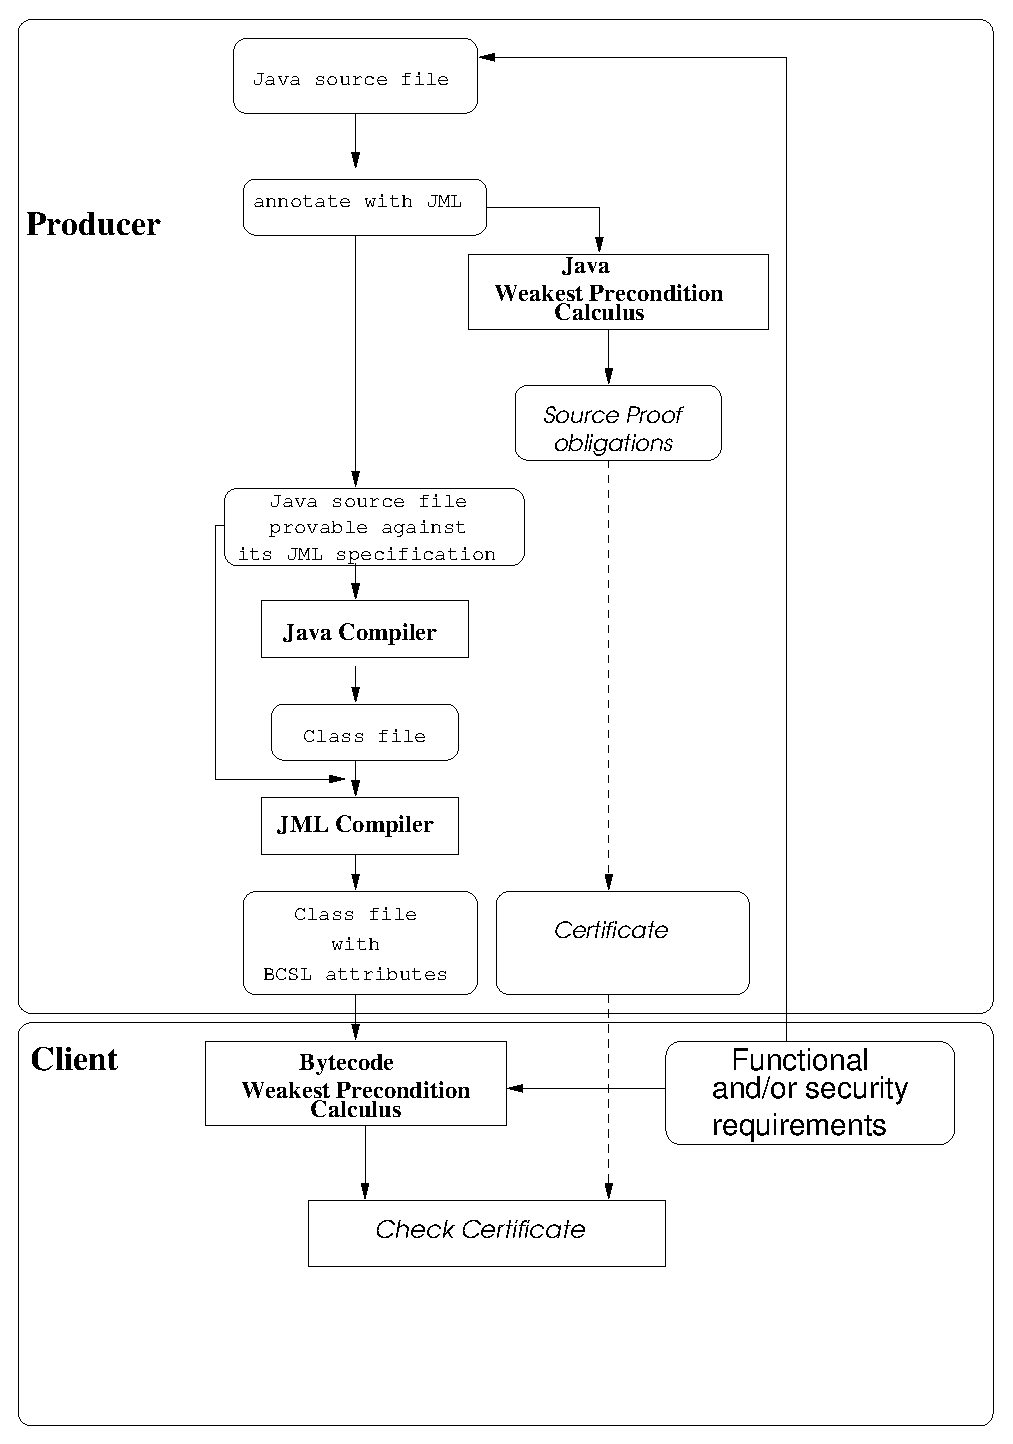
\psfig{file=../Papers/isaac/architecture.eps,width=\textwidth}
\end{slide}

\begin{slide}{Assertion generation}
Two phases:
\begin{itemize}
\item \Blue{synthesising} core-annotations
\item \Blue{weaving} annotations throughout the application
\end{itemize}
\ \smallskip\\
\Blue{Synthesising}: for each property annotations have to be defined
\bigskip\\
\Blue{Weaving}: algorithm for pre- and postcondition generation
\end{slide}

\begin{slide}{Example core-annotations}
\Red{No nested transactions}
\begin{alltt}
\Blue{\textbf{/*@ static ghost int TRANSACT == 0; @*/}}
\end{alltt}
\ \smallskip\\
Method \textttbf{beginTransaction}
\begin{alltt}
\Blue{\textbf{/*@ requires TRANSACT == 0;
  @ assignable TRANSACT;
  @ ensures TRANSACT == 1; @*/}}
\textbf{public static native 
   void beginTransaction() 
        throws TransactionException;}
\end{alltt}
\ \smallskip\\
Similar annotations for \textttbf{commitTransaction},
\textttbf{abortTransaction} 
\end{slide}


\begin{slide}{Preconditions for methods}
\begin{alltt}
\textbf{public void m() \{
   ...
   \Blue{// will require TRANSACT == 0}
   JCSystem.beginTransaction();
   \Blue{// TRANSACT modified, 
   // ensures TRANSACT == 1}
   ...
   \Blue{// will require TRANSACT == 1}
   JSSystem.commitTransaction();
   \Blue{// TRANSACT modified, 
   // ensures TRANSACT == 0}
   ...
   \}}
\end{alltt}
\end{slide}


\begin{slide}{Preconditions for methods}
\vspace*{-1em}
\begin{alltt}
\textbf{\Red{/*@ requires \texttt{TRANSACT == 0} */}}
\textbf{public void m() \{
   ...
   \Blue{// will require TRANSACT == 0}
   JCSystem.beginTransaction();
   \Blue{// TRANSACT modified, 
   // ensures TRANSACT == 1}
   ...
   \Blue{// will require TRANSACT == 1}
   JSSystem.commitTransaction();
   \Blue{// TRANSACT modified, 
   // ensures TRANSACT == 0}
   ...
   \}}
\end{alltt}
\end{slide}

\begin{slide}{Some assumptions we make}
\begin{itemize}
  \item Only variables in annotations are static and ghost of primitive type
  \item Appropriate modelling of programs
  \item Existence of function {\large\textsf{\Red{mod}}}: set of static ghost
variables modified by statement 
\end{itemize}
\end{slide}

\begin{slide}{Algorithm for precondition generation}
\begin{itemize}
   \item \Blue{Method declaration}
\[\mathsf{\OliveGreen{pre}}(m)  =  \mathsf{\OliveGreen{pre}}(\mathsf{body}(m), \emptyset)\]
   \item \Blue{Composition}
\[\mathsf{\OliveGreen{pre}}(s_1 \mathtt{;} s_2, V)  =  \mathsf{\OliveGreen{pre}}(s_1, V) \cup 
                                          \mathsf{\OliveGreen{pre}}(s_2, V \cup
\mathsf{\Red{mod}}(s1))\]
   \item \Blue{Method call}
\[\mathsf{\OliveGreen{pre}}(\mathsf{\Blue{call}}(n),V)  =  
                \{ p \mid p \in \mathsf{\OliveGreen{pre}}(n) \wedge 
                          \mathsf{fv}(p) \cap V = \emptyset\}\]
\end{itemize}
\end{slide}

\begin{slide}{Algorithm for precondition generation - branching statements}
\begin{itemize}
   \item \Blue{Conditional}
\[
\mathsf{\OliveGreen{pre}}(\mathtt{if\:(} c \mathtt{)\:} s_1 \mathtt{\:else\:} s_2,
V)  = 
\begin{array}[t]{l}
   \mathsf{\OliveGreen{pre}}(c, V) \:\cup \\
   \mathsf{\OliveGreen{pre}}(s_1, V \cup \mathsf{\Red{mod}}(c)) \:\cup\\
   \mathsf{\OliveGreen{pre}}(s_2, V \cup \mathsf{\Red{mod}}(c))
\end{array}\]
\item \Blue{Try catch}
\[\mathsf{\OliveGreen{pre}}(\mathtt{try\:} s_1 \mathtt{\:catch\:(} E \mathtt{)\:} s_2, V)  =  \begin{array}[t]{l}
   \mathsf{\OliveGreen{pre}}(s_1, V) \:\cup \\
   \mathsf{\OliveGreen{pre}}(s_2, V \cup \mathsf{\Red{mod}}(s1))
  \end{array}\]
\end{itemize}
\end{slide}




\begin{slide}{Experiments: checking atomicity properties}

\Red{No uncaught exceptions in transactions}\smallskip\\

\begin{alltt}
\textbf{\Blue{/*@ exsures (Exception) TRANSACT == 0; @*/}
public static native void 
   commitTransaction() 
         throws TransactionException;}
\end{alltt}
\ \medskip\\
Annotation propagated to each statement block, ending with commit.
\end{slide}

\begin{slide}{Experiments: checking atomicity properties}
\Red{No pin-verification within transaction}\smallskip\\

\begin{alltt}
\textbf{\Blue{/*@ requires TRANSACT == 0; @*/}
public boolean check(byte[] pin, 
                     short offset, 
                     byte length);}
\end{alltt}
\end{slide}

\begin{slide}{Results}
\begin{itemize}
\item Tested on several realistic smart card applications
\item One core-annotation can give rise to many annotations in
different classes (26 annotations, spread over 5 different classes)
\item Several violations found: uncaught exceptions possible within
transactions 
\end{itemize}
\end{slide}

\begin{slide}{Uncaught exception within transaction}
\begin{alltt}
\textbf{void appExchangeCurrency(...) \{
   ...
   \Blue{/*@ exsures (Exception) TRANSACT == 0; @*/} \{
      ...
      JCSystem.beginTransaction();	
      try \{balance.setValue(decimal2);
            ...
      \} catch (DecimalException e) \{
         ISOException.throwIt(
              PurseApplet.OVERFLOW);
      \}
      JCSystem.commitTransaction();
   \}
   ...\}}
\end{alltt}
\end{slide}


\begin{slide}{Towards more generality:\\ Security automata}
\begin{itemize}
\item \Blue{Security automaton}: monitors program behaviour,
blocking/error upon unwanted behaviour 
\item Use security automata to express security properties
\item Automatic generation of core-annotations
\item Use any JML tool to check whether program respects the property
\end{itemize}
\end{slide}

\overlays{2}{
\begin{slide}{Correctness}
\begin{center}
\Blue{If program satisfies annotations \\
      then it respects the security property}
\end{center}
\ \smallskip\\
\FromSlide{2}
\begin{itemize}
\item First soundness proof for simple while-language on the way
\item In some cases also completeness
\end{itemize}
\end{slide}
}

\overlays{3}{
\begin{slide}{If program satisfies annotations \\
      then it respects the security property}
Approach:
\begin{itemize}
\item If fully annotated program verified, run-time monitoring it (with
\texttt{jmlc}) will not block  \\
\OliveGreen{\(P \models_{ST} \mathsf{prop}(P, \mathsf{core}(\mathcal{T})) \Rightarrow
P \models_{RV} \mathsf{prop}(P, \mathsf{core}(\mathcal{T}))\)}
\FromSlide{2}\item If fully annotated program run-time okay,
core-annotated program run-time okay\\
\OliveGreen{\(P \models_{RV} \mathsf{prop}(P, \mathsf{core}(\mathcal{T})) \Rightarrow
P \models_{RV} \mathsf{core}(\mathcal{T})\)}
\FromSlide{3}\item If core-annotated program run-time okay,security
automaton  will not block\\
\OliveGreen{\(P \models_{RV} \mathsf{core}(\mathcal{T}) \Rightarrow \mathcal{OK}(P \times
\mathcal{T})\)}
\end{itemize}
\end{slide}
}

\begin{slide}{Completeness?}
\begin{itemize}
\item 
\OliveGreen{\(P \models_{ST} \mathsf{prop}(P, \mathsf{core}(\mathcal{T})) \Red{\Leftrightarrow}
P \models_{RV} \mathsf{prop}(P, \mathsf{core}(\mathcal{T}))\)}
\item
\OliveGreen{\(P \models_{RV} \mathsf{core}(\mathcal{T}) \Red{\Leftrightarrow} \mathcal{OK}(P \times
\mathcal{T})\)}
\item But what about propagation:
\Red{\(P \models_{RV} \mathsf{prop}(P, \mathsf{core}(\mathcal{T})) \Leftarrow
P \models_{RV} \mathsf{core}(\mathcal{T})\)} ??
\end{itemize}
\end{slide}

\begin{slide}{Example: propagation does not preserve run-time verification}

\begin{alltt}
\textbf{\phantom{\Red{/*@ requires TRANSACT == 0; */}}
void m() \{
  if (false) \{ \Blue{// requires TRANSACT == 0;}
               beginTransaction();\}
\}

void n() \{
  beginTransaction();
  \Blue{// ensures TRANSACT == 1;}
  m();
\}}
\end{alltt}
\ \smallskip\\
Run-time verification ok
\end{slide}

\begin{slide}{Example: propagation does not preserve run-time verification}

\begin{alltt}
\textbf{\Red{/*@ requires TRANSACT == 0; */}
void m() \{
  if (false) \{ \Blue{// requires TRANSACT == 0;}
               beginTransaction();\}
\}

void n() \{
  beginTransaction();
  \Blue{// ensures TRANSACT == 1;}
  m();
\}}
\end{alltt}
\ \smallskip\\
Run-time verification signals error
\end{slide}

\begin{slide}{Conditional completeness?}
Run-time verification preserved by propagation, if:
\begin{itemize}
\item Program does not contain branching statements
\item Branching statements do not propagate any annotations
\item Each branch of statement propagates same annotations ??
\end{itemize}
\end{slide}

\begin{slide}{Future issues}
\begin{itemize}
\item Other formalisms to express security properties (with
translation into JML)?
\item Translations into other formalisms
\item Do we need liveness?
\end{itemize}
\end{slide}

\begin{slide}{Theoretical foundations: abstract weakest precondition}
Abstract wp-calculus \OliveGreen{\(\mathsf{wp}^\#\)}: considers only static 
ghost variables\\
Example rules:
\[
\begin{array}{l}
\mathsf{\OliveGreen{wp}}^{\OliveGreen{\#}}(\mathtt{if
(}c\mathtt{)}s_1\mathtt{\:else\:}s_2,Q) =\\
\qquad
\mathsf{\OliveGreen{wp}}^{\OliveGreen{\#}}(c, \mathsf{\OliveGreen{wp}}^{\OliveGreen{\#}}(s_1, Q)) \wedge
\mathsf{\OliveGreen{wp}}^{\OliveGreen{\#}}(c,
\mathsf{\OliveGreen{wp}}^{\OliveGreen{\#}}(s_2, Q))
\end{array}
\]

\[
\mathsf{\OliveGreen{wp}}^{\OliveGreen{\#}}(\mathsf{\Blue{call}}(m), Q) =
  \mathsf{\Blue{requires}}(m) \wedge 
  \forall \mathsf{\Red{mod}}(m). (\mathsf{\Blue{ensures}}(m) \Rightarrow Q)
\]
\end{slide}

\begin{slide}{Results}
\begin{itemize}
\item Any proof in abstract wp-calculus, is proof in standard
wp-calculus
\[
\forall P, Q\colon\mathsf{Pred}, s\colon\mathsf{Stmt}. 
(P \Rightarrow \mathsf{\OliveGreen{wp}}^{\OliveGreen{\#}}(s, Q)) \Rightarrow
               (P \Rightarrow \mathsf{\OliveGreen{wp}}(s, Q))
\]
\item Precondition generation computes the \emph{free} part of the
abstract weakest precondition
\[
\exists F\colon\mathsf{Pred}.  
             \mathsf{\OliveGreen{wp}}^{\OliveGreen{\#}}(s, \lambda x. \mathsf{true}) = 
             (\mathsf{\OliveGreen{pre}}(s, \emptyset) \wedge \forall
              \mathsf{\Red{mod}}(s). F) 
\]
\end{itemize}
\end{slide}

\end{document}